\documentclass{article}

\usepackage[english]{babel}

% Set page size and margins
% Replace `letterpaper' with`a4paper' for UK/EU standard size
\usepackage[letterpaper,top=2cm,bottom=2cm,left=3cm,right=3cm,marginparwidth=1.75cm]{geometry}

% Useful packages
\usepackage{amsmath}
\usepackage{graphicx}
\usepackage[colorlinks=true, allcolors=blue]{hyperref}

%\usepackage{caption}
%\usepackage{subcaption}
\usepackage{subfig}

\title{Preliminary Analysis of Stroke Participant's Movement}
\author{Milli Schlafly}

\begin{document}
\maketitle

Analysis notes:
\begin{itemize}
	\item Movement when the ball is green is removed. (Only matters for 1 or 2 participants)
	\item Movement when participant is not lifted is removed. (Negligible effect on results)
	\item Window of +/- 0.3Hz
\end{itemize}

Ball frequency is a significant factor in nearly every ANOVA that was performed. Because this result could be due to factors other than the participant's ability to produce motion at the ball's resonant frequency, I do not note if ball frequency is significant in this document. 


\section{Overall results}

\begin{figure}[!ht]
     \centering
     \subfloat{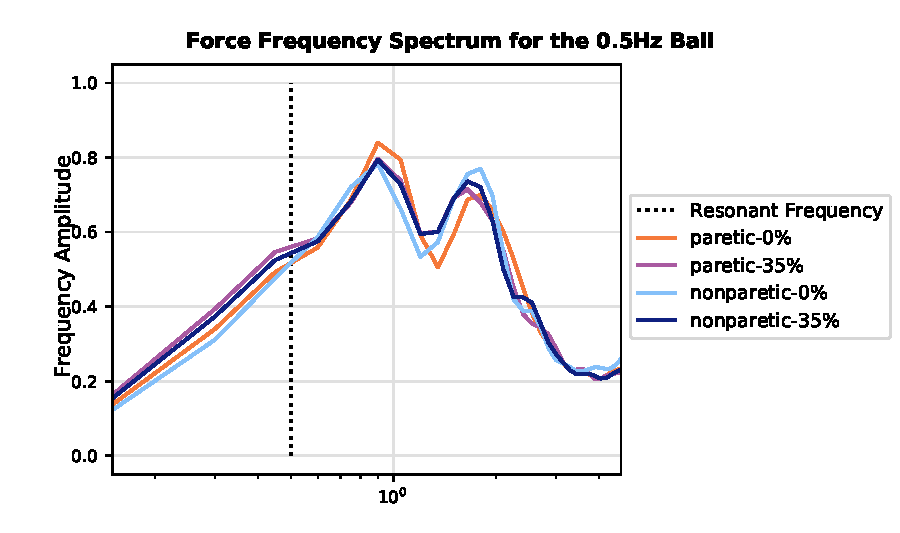
\includegraphics[width=0.5\linewidth]{Plots/agg_spectrum_0.5Hz.pdf}}
     \subfloat{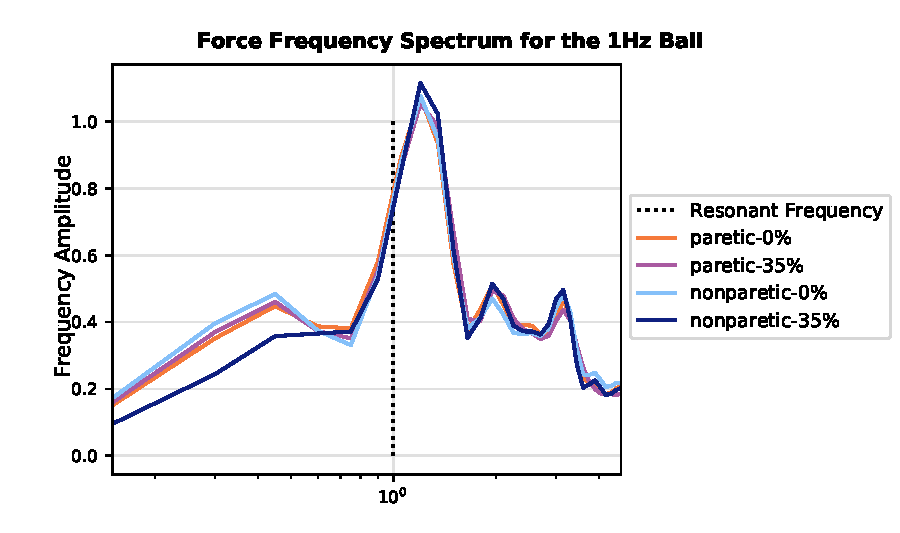
\includegraphics[width=0.5\linewidth]{Plots/agg_spectrum_1Hz.pdf}}
     \hfill
     \subfloat{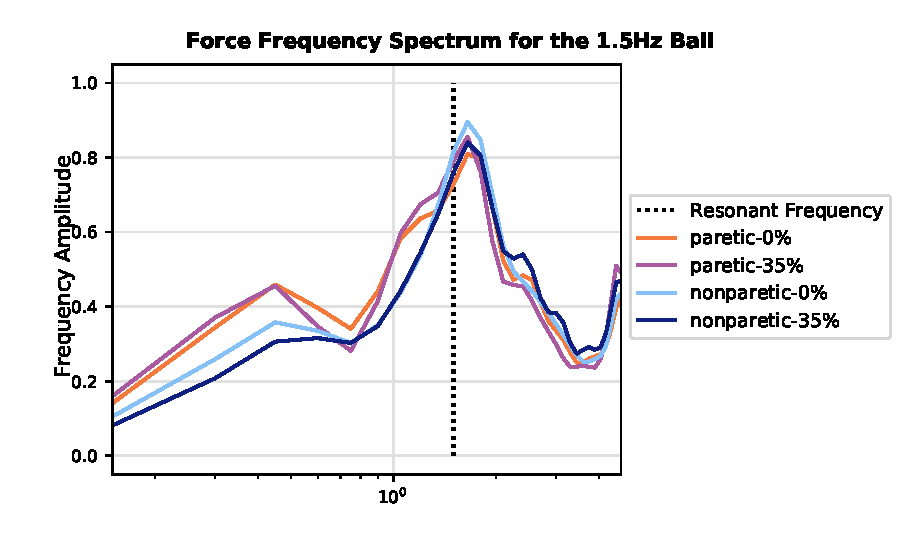
\includegraphics[width=0.5\linewidth]{Plots/agg_spectrum_1.5Hz.pdf}}
     \subfloat{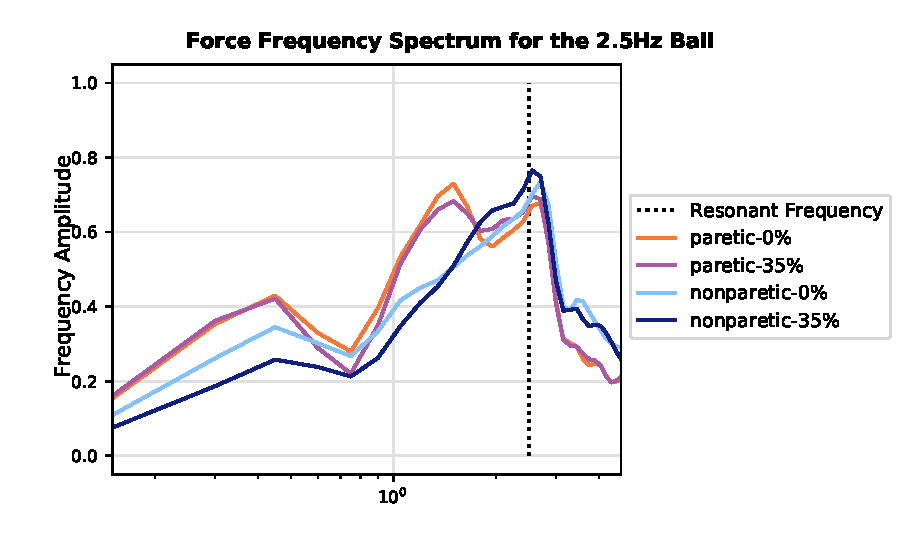
\includegraphics[width=0.5\linewidth]{Plots/agg_spectrum_2.5Hz.pdf}}
     \hfill
	\caption{Aggregate Frequency Spectrums. With the 1.5Hz and 2.5Hz ball, participants struggled to reach the resonant frequency with their paretic arm, resulting in a mound (or, for 2.5Hz, a second peak) below the resonant frequency. No trends are apparent trends at 0.5Hz}
\end{figure}

\begin{figure}[!ht]
     \centering
     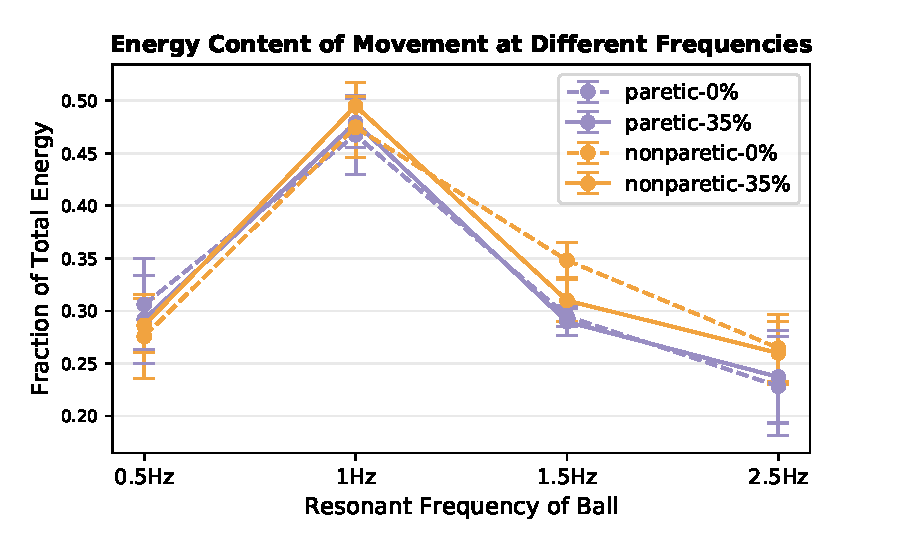
\includegraphics[width=0.5\linewidth]{Plots/e_at_res_raw.pdf}
	\caption{Energy at the resonant frequency of the ball metric. Arm is close to significance (p=0.093). The interaction effect between arm and ball frequency is close to significance (p=0.083). For the 1.5Hz ball, arm has a significant effect on the energy at resonance (p=0.013). For the 2.5Hz ball, arm almost has a significant effect on the energy at resonance (p=0.058).}
\end{figure}


\begin{figure}[!ht]
     \centering
     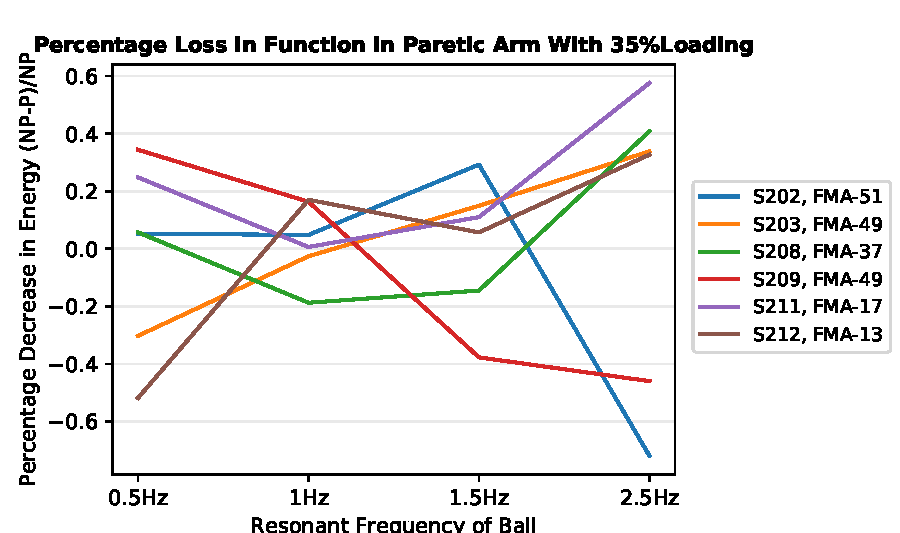
\includegraphics[width=0.5\linewidth]{Plots/pl_SL1_seperate.pdf}
	\caption{Percent loss in paretic arm with loading. Positive values indicate better performance in the nonparetic arm. Negative values indicate better performance in the paretic arm. A positive trend is observed for 4/6 participants. The remaining participants, S202 and S209 who are more mildly impaired, exhibit the opposite trend. No statistical significance.}
\end{figure}

\begin{figure}[!ht]
     \centering
     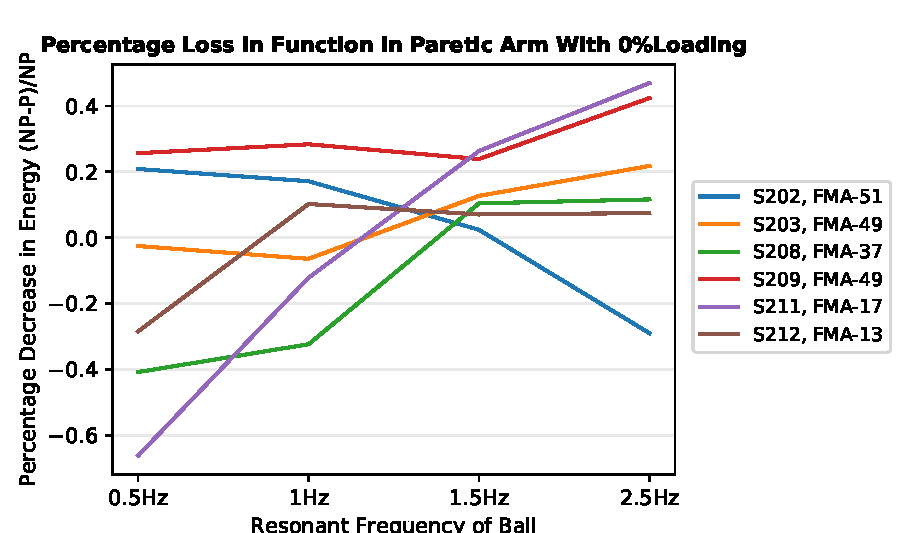
\includegraphics[width=0.5\linewidth]{Plots/pl_SL0_seperate.pdf}
	\caption{Percent loss in paretic arm with no loading. Positive values indicate better performance in the nonparetic arm. Negative values indicate better performance in the paretic arm. A positive trend is observed for 5/6 participants. No statistical significance.}
\end{figure}


\begin{figure}[!ht]
     \centering
     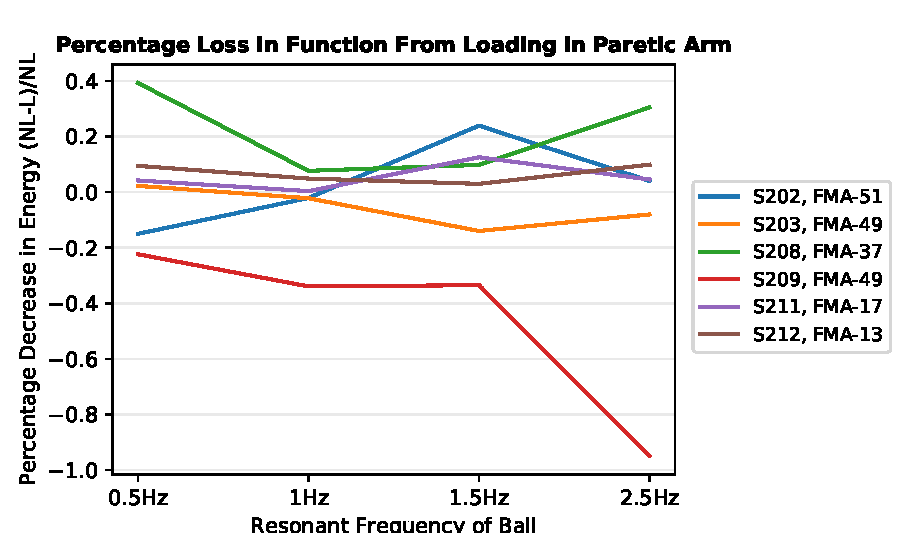
\includegraphics[width=0.5\linewidth]{Plots/pl_A0_seperate.pdf}
	\caption{Percent loss in function in the paretic arm due to loading. Positive values indicate better performance during no loading. Negative values indicate better performance with loading. No trend w.r.t. frequency is apparent. Values are generally positive, indicating better performance without loading. No statistical significance.}
\end{figure}


\begin{figure}[!ht]
     \centering
     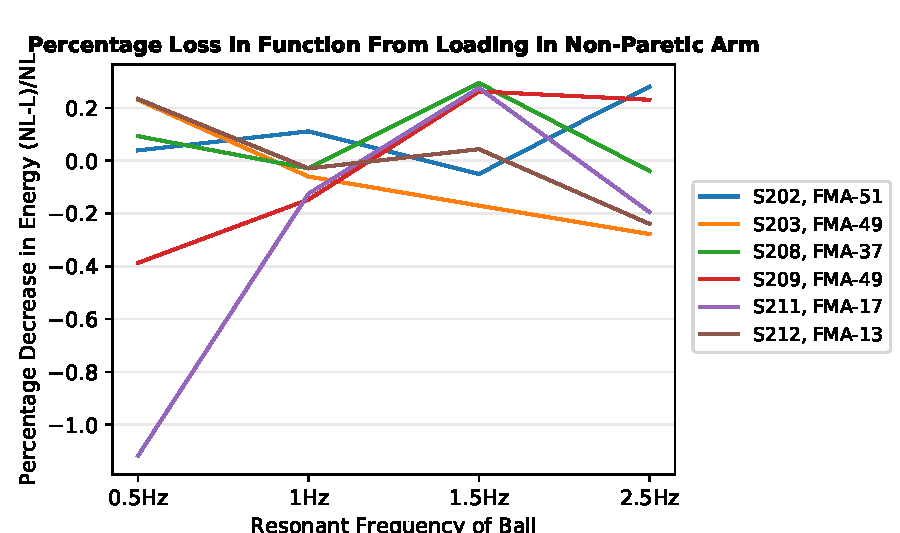
\includegraphics[width=0.5\linewidth]{Plots/pl_A1_seperate.pdf}
	\caption{Percent loss in function in the paretic arm due to loading. Positive values indicate better performance during no loading. Negative values indicate better performance with loading. No trend is apparent. No statistical significance.}
\end{figure}


\clearpage
\section{Individual Subject Results}

\subsection{S202; FMA = 51}

\begin{figure}[!ht]
     \centering
     \subfloat{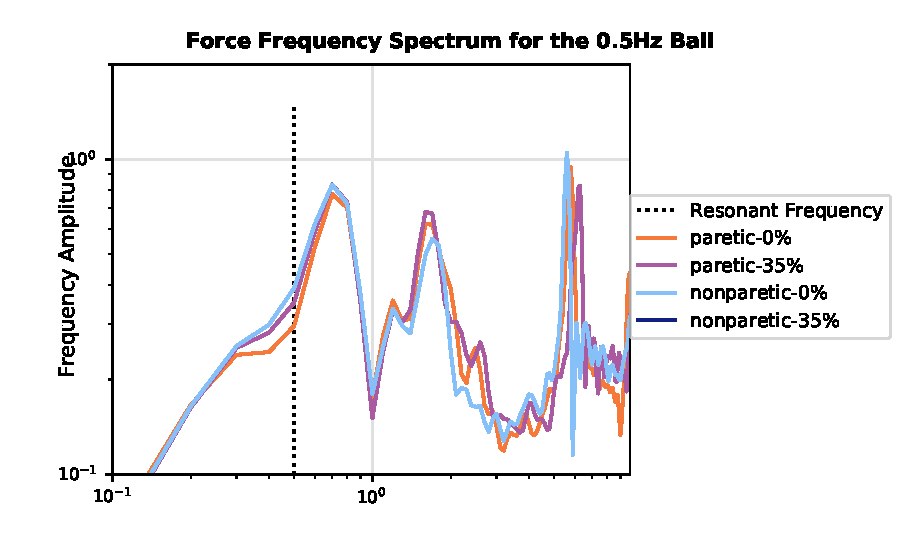
\includegraphics[width=0.5\linewidth]{Plots/IndividualSubjectPlots/S202/S202_0.5Hz.pdf}}
     \subfloat{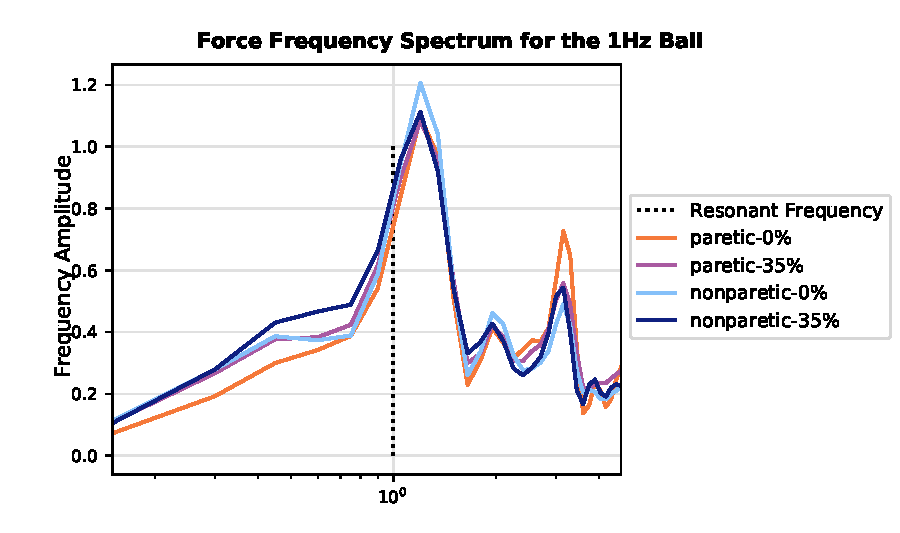
\includegraphics[width=0.5\linewidth]{Plots/IndividualSubjectPlots/S202/S202_1Hz.pdf}}
     \hfill
     \subfloat{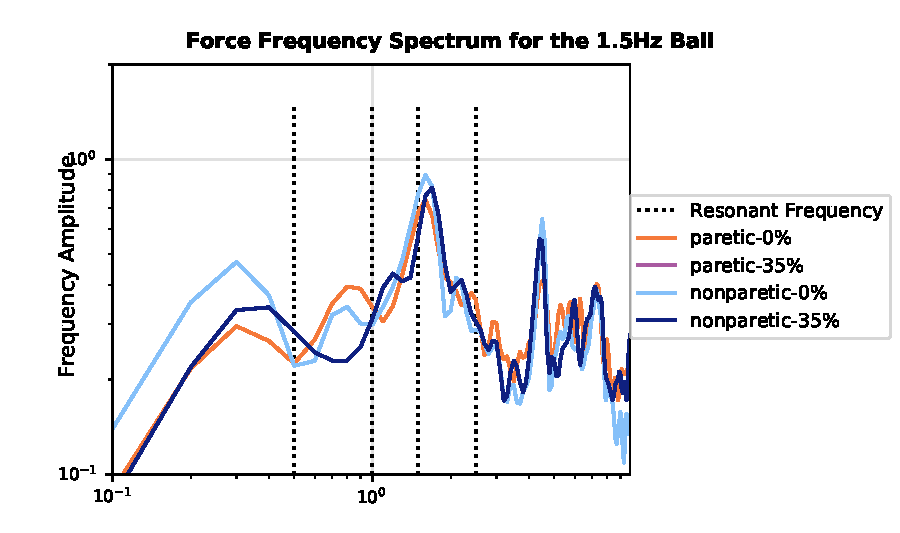
\includegraphics[width=0.5\linewidth]{Plots/IndividualSubjectPlots/S202/S202_1.5Hz.pdf}}
     \subfloat{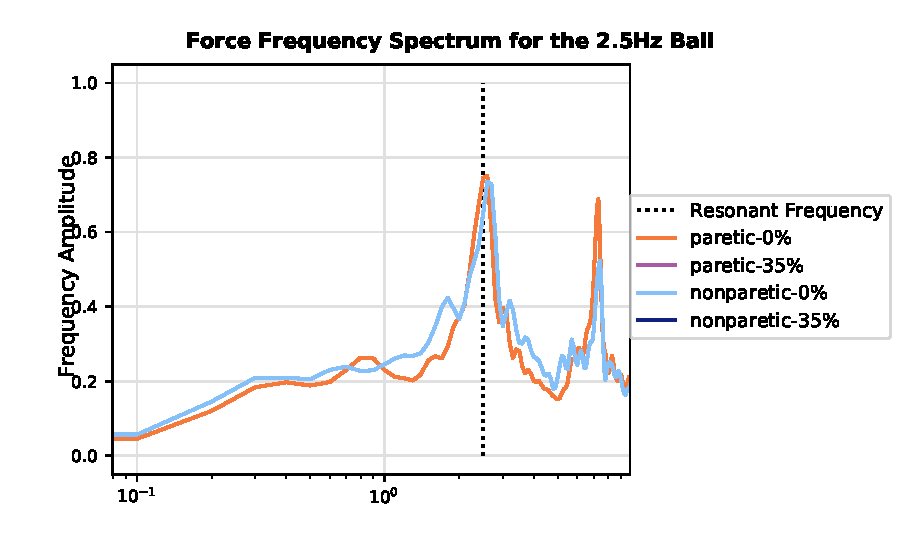
\includegraphics[width=0.5\linewidth]{Plots/IndividualSubjectPlots/S202/S202_2.5Hz.pdf}}
     \hfill
     \subfloat{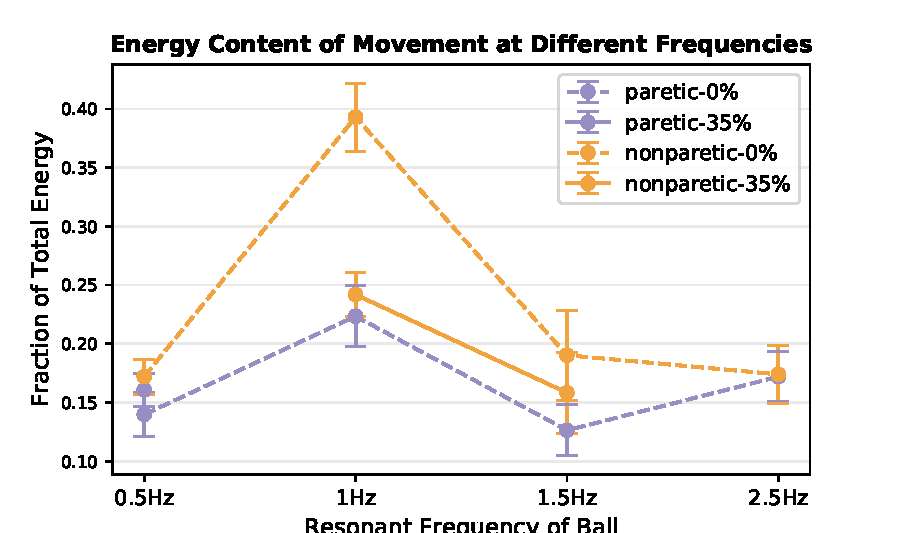
\includegraphics[width=0.5\linewidth]{Plots/IndividualSubjectPlots/S202/S202.pdf}}
	\caption{Subject 202 Frequency Spectrums. Interation effect between arm and ball frequency (p$<$0.001). P-values for factor arm is significant for 2.5Hz ball. For the 1.5Hz ball, loading is a significant factor in the paretic arm. For the 2.5Hz ball, loading is a significant factor in the nonparetic arm. Ball frequency is a significant factor for percent decrease in paretic arm with loading  with 2.5Hz being different.}
\end{figure}

\clearpage
\subsection{S203; FMA = 49}

\begin{figure}[!ht]
     \centering
     \subfloat{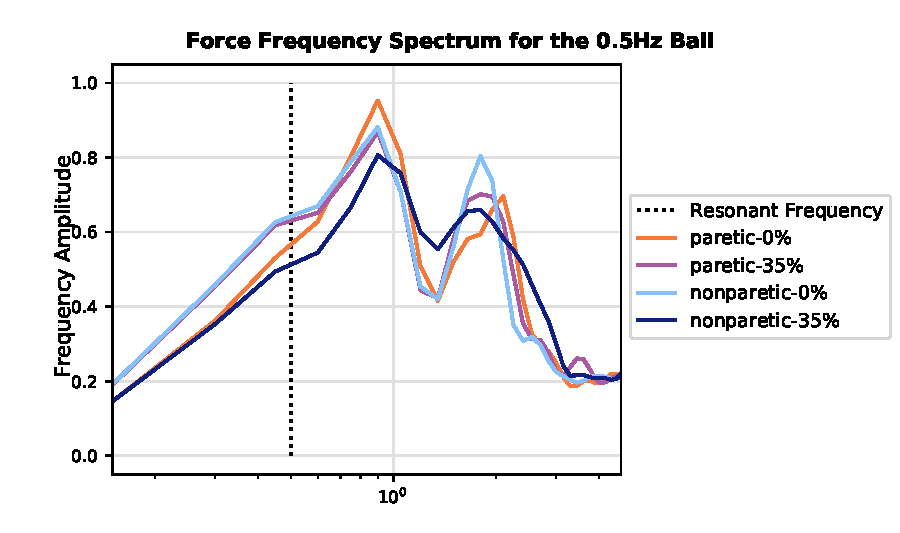
\includegraphics[width=0.5\linewidth]{Plots/IndividualSubjectPlots/S203/S203_0.5Hz.pdf}}
     \subfloat{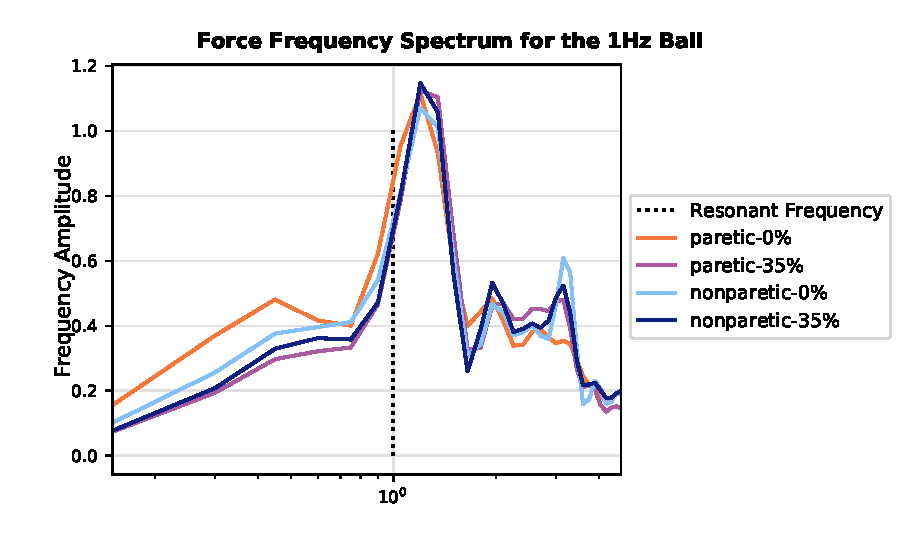
\includegraphics[width=0.5\linewidth]{Plots/IndividualSubjectPlots/S203/S203_1Hz.pdf}}
     \hfill
     \subfloat{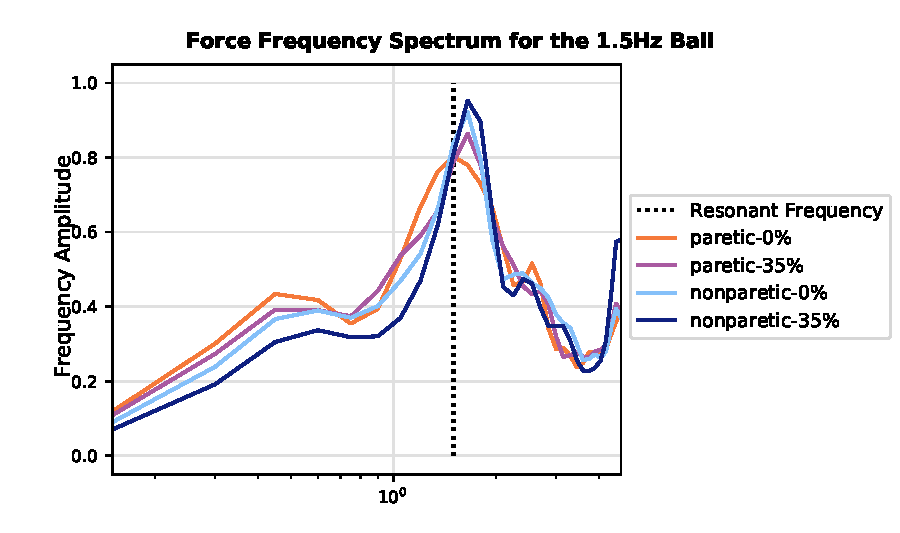
\includegraphics[width=0.5\linewidth]{Plots/IndividualSubjectPlots/S203/S203_1.5Hz.pdf}}
     \subfloat{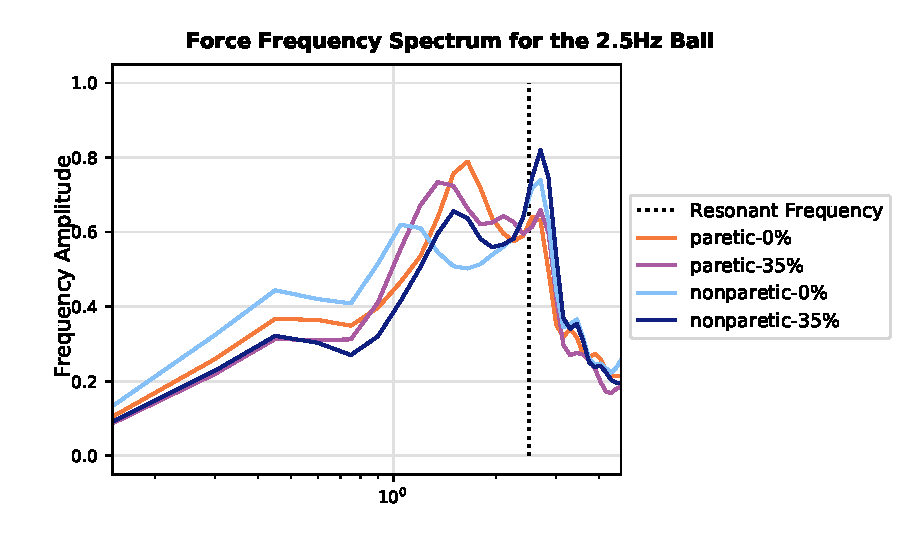
\includegraphics[width=0.5\linewidth]{Plots/IndividualSubjectPlots/S203/S203_2.5Hz.pdf}}
     \hfill
     \subfloat{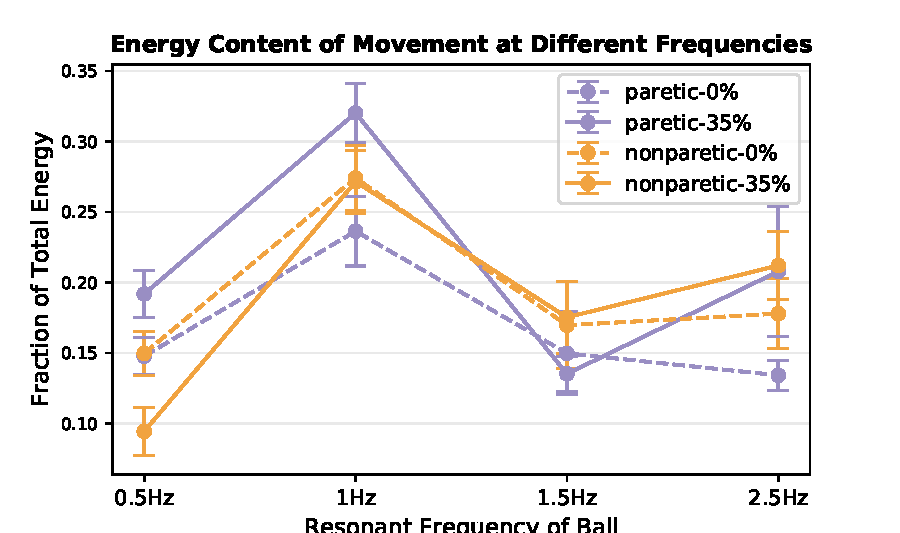
\includegraphics[width=0.5\linewidth]{Plots/IndividualSubjectPlots/S203/S203.pdf}}
	\caption{Subject 203 Frequency Spectrums. Interation effect between arm and ball frequency (p$<$0.01). For the 2.5Hz ball, arm is a significant factor. Ball frequency is a significant factor for percent decrease in paretic arm with loading  with 0.5Hz being different.}
\end{figure}

\clearpage
\subsection{S205; FMA = 34}

The participant was not able to match the resonant frequency of the 1.5Hz and 2.5Hz balls with their nonparetic limb. Therefore, this participant was removed from the aggregate analyses.

\begin{figure}[!ht]
     \centering
     \subfloat{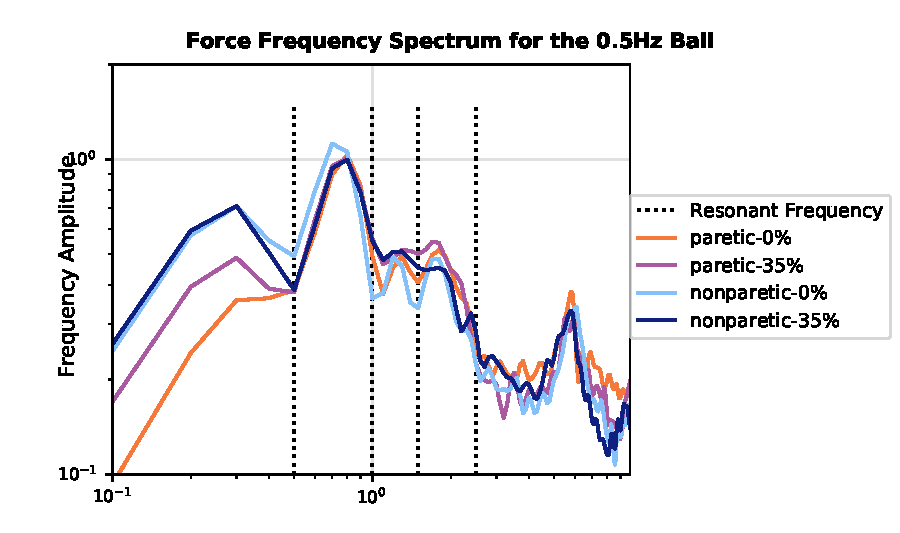
\includegraphics[width=0.5\linewidth]{Plots/IndividualSubjectPlots/S205/S205_0.5Hz.pdf}}
     \subfloat{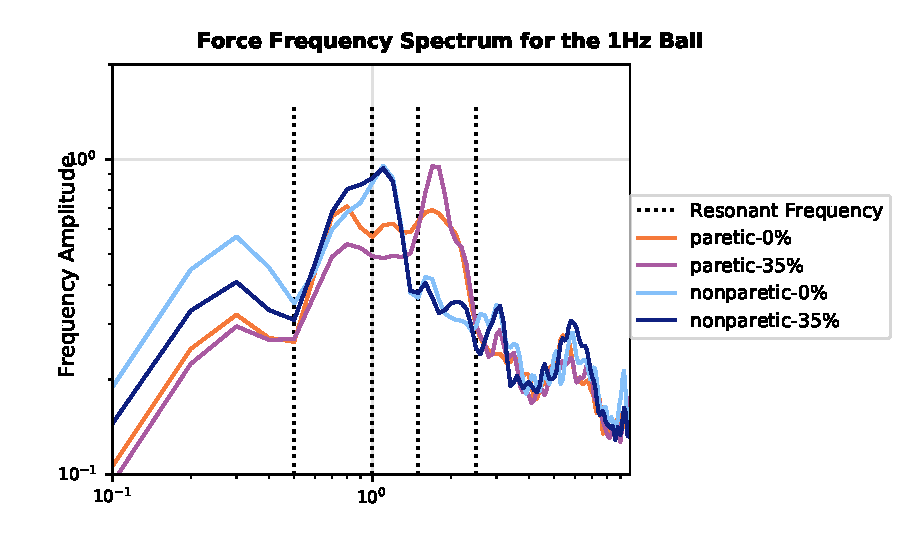
\includegraphics[width=0.5\linewidth]{Plots/IndividualSubjectPlots/S205/S205_1Hz.pdf}}
     \hfill
     \subfloat{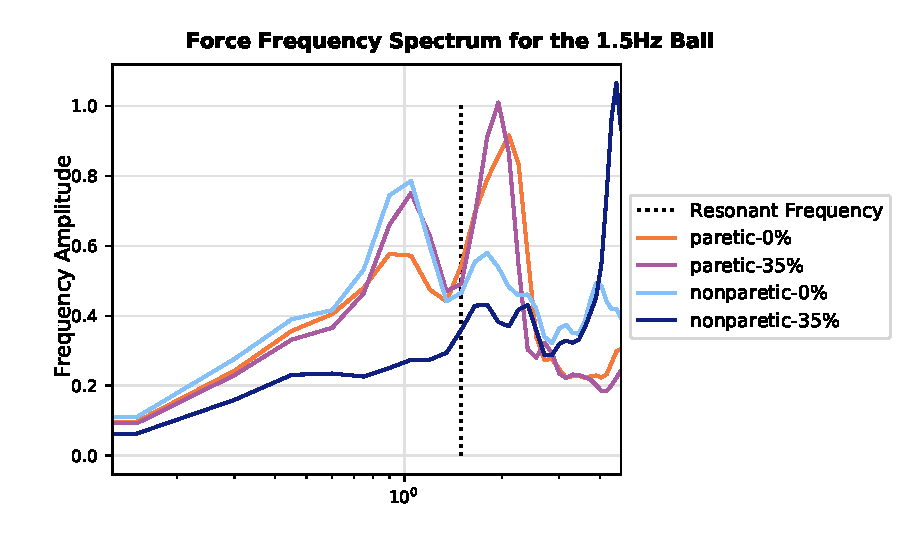
\includegraphics[width=0.5\linewidth]{Plots/IndividualSubjectPlots/S205/S205_1.5Hz.pdf}}
     \subfloat{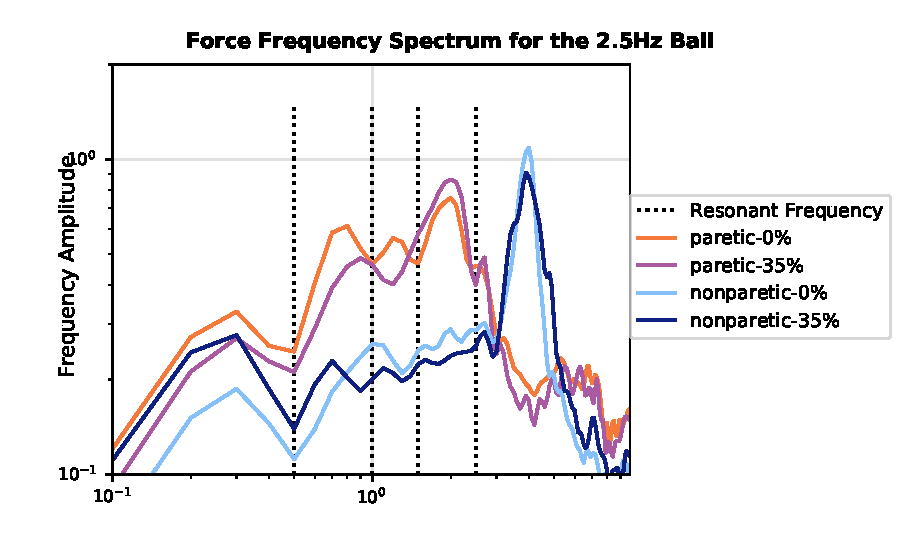
\includegraphics[width=0.5\linewidth]{Plots/IndividualSubjectPlots/S205/S205_2.5Hz.pdf}}
     \hfill
     \subfloat{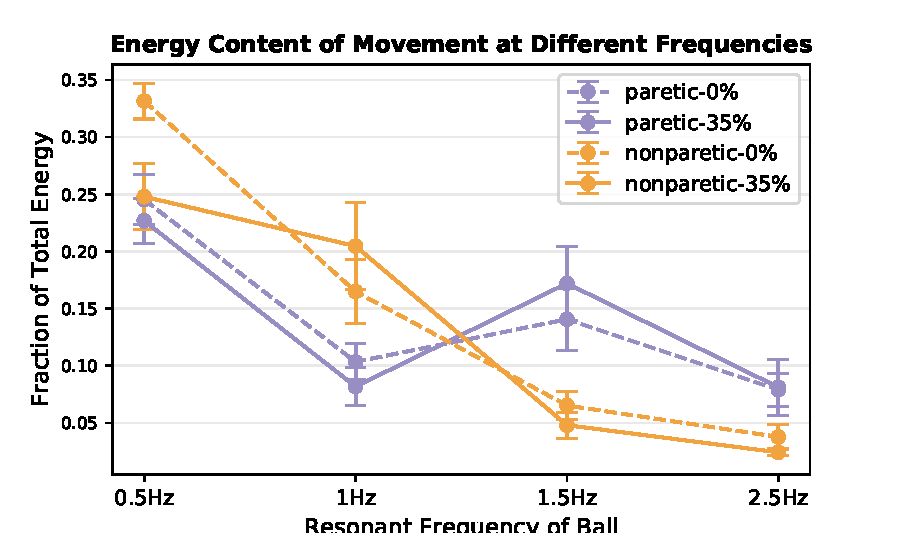
\includegraphics[width=0.5\linewidth]{Plots/IndividualSubjectPlots/S205/S205.pdf}}
	\caption{Subject 205 Frequency Spectrums}
\end{figure}

\clearpage
\subsection{S207; FMA = 30}

The participant was not able to match the resonant frequency of the 1.5Hz and 2.5Hz balls with their nonparetic limb. Therefore, this participant was removed from the aggregate analyses.

\begin{figure}[!ht]
     \centering
     \subfloat{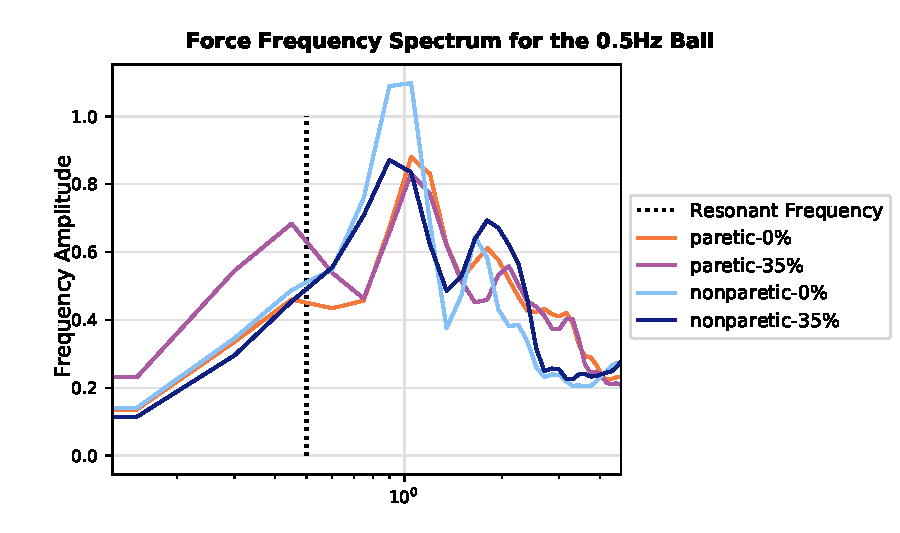
\includegraphics[width=0.5\linewidth]{Plots/IndividualSubjectPlots/S207/S207_0.5Hz.pdf}}
     \subfloat{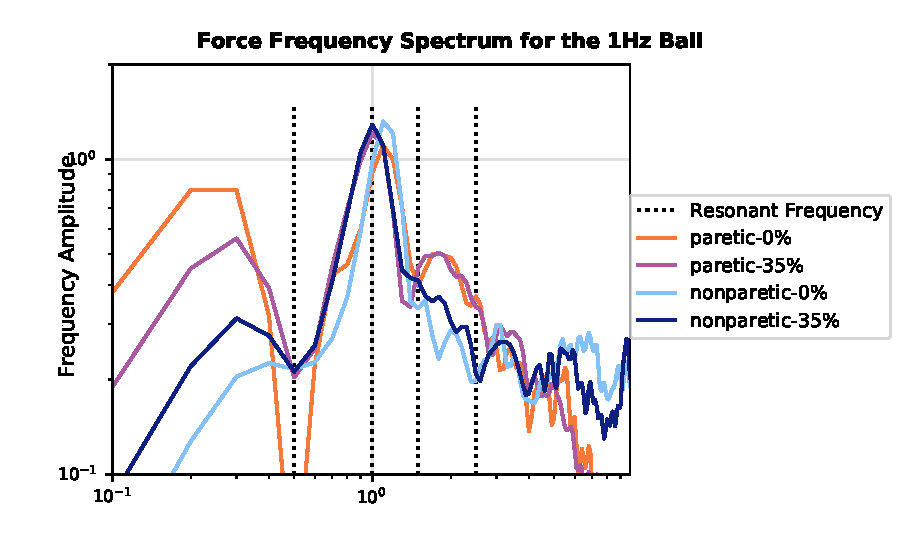
\includegraphics[width=0.5\linewidth]{Plots/IndividualSubjectPlots/S207/S207_1Hz.pdf}}
     \hfill
     \subfloat{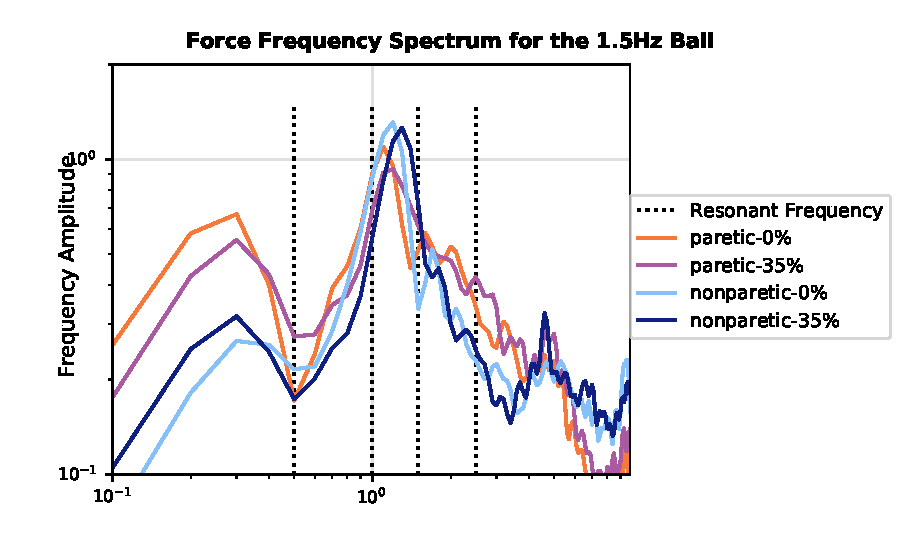
\includegraphics[width=0.5\linewidth]{Plots/IndividualSubjectPlots/S207/S207_1.5Hz.pdf}}
     \subfloat{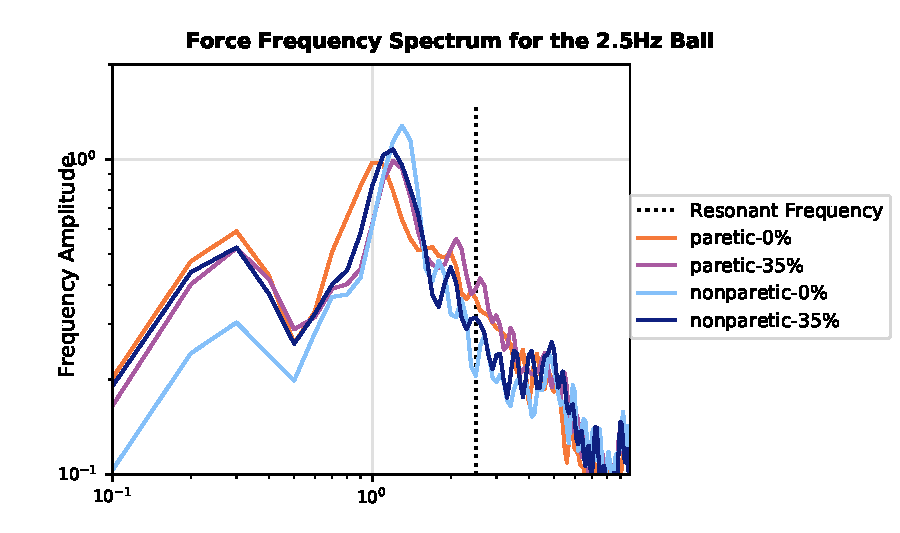
\includegraphics[width=0.5\linewidth]{Plots/IndividualSubjectPlots/S207/S207_2.5Hz.pdf}}
     \hfill
     \subfloat{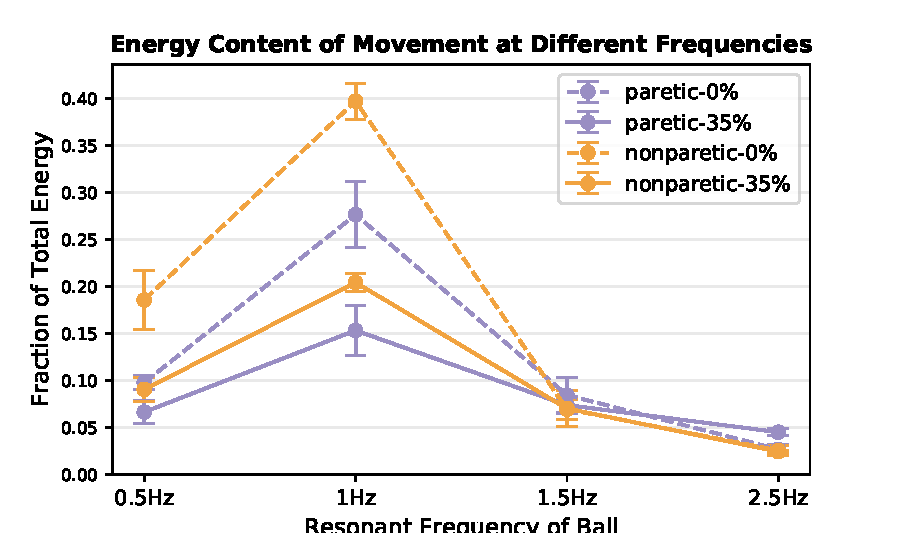
\includegraphics[width=0.5\linewidth]{Plots/IndividualSubjectPlots/S207/S207.pdf}}
	\caption{Subject 207 Frequency Spectrums}
\end{figure}

\clearpage
\subsection{S208; FMA = 37}

\begin{figure}[!ht]
     \centering
     \subfloat{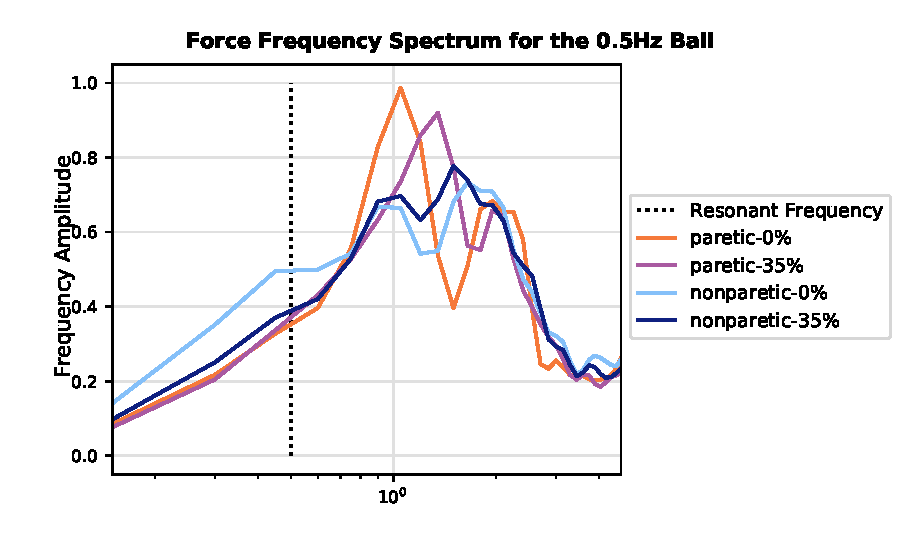
\includegraphics[width=0.5\linewidth]{Plots/IndividualSubjectPlots/S208/S208_0.5Hz.pdf}}
     \subfloat{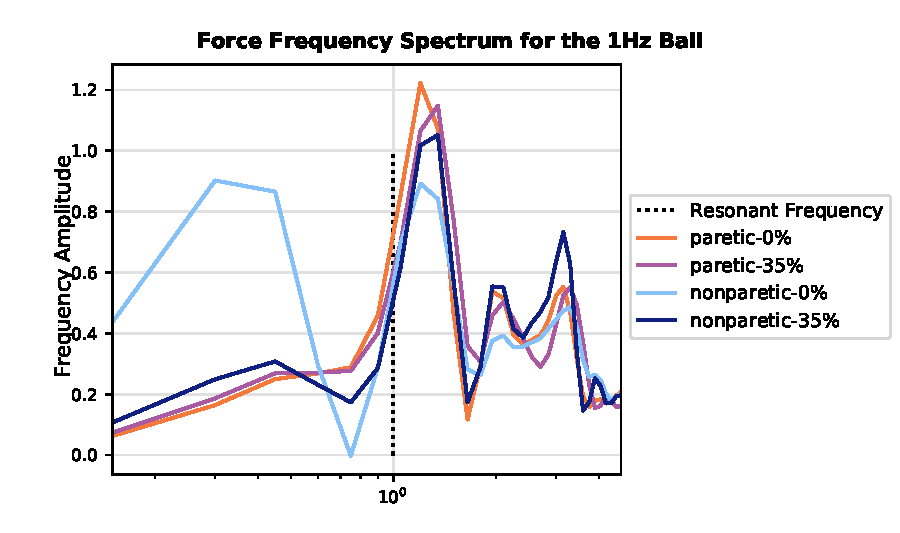
\includegraphics[width=0.5\linewidth]{Plots/IndividualSubjectPlots/S208/S208_1Hz.pdf}}
     \hfill
     \subfloat{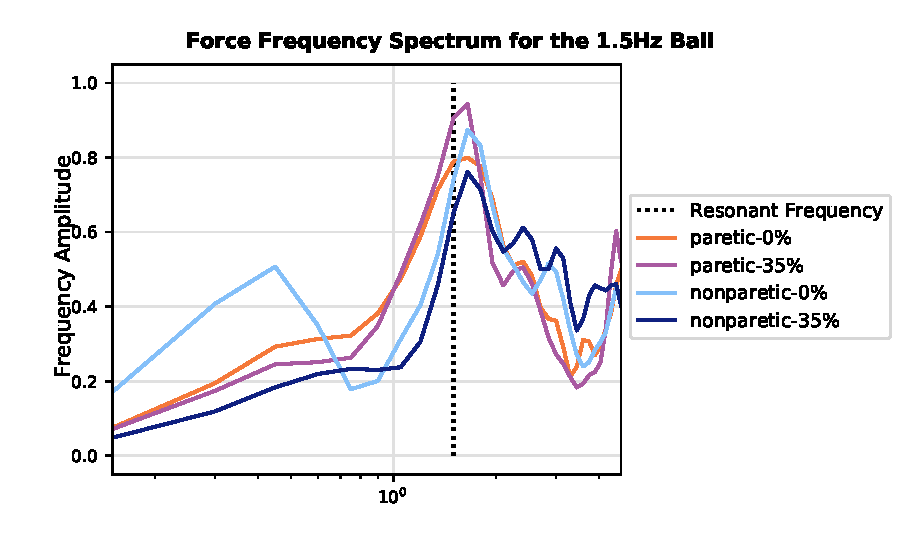
\includegraphics[width=0.5\linewidth]{Plots/IndividualSubjectPlots/S208/S208_1.5Hz.pdf}}
     \subfloat{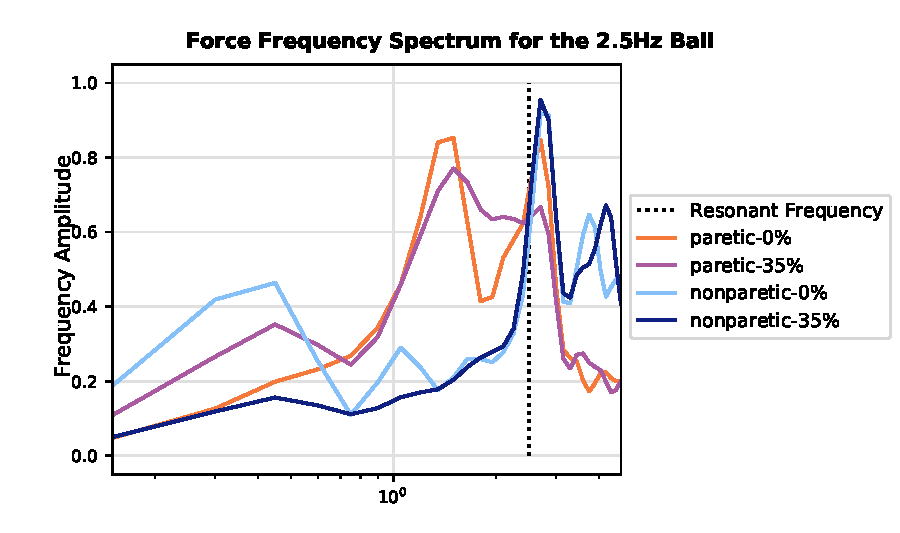
\includegraphics[width=0.5\linewidth]{Plots/IndividualSubjectPlots/S208/S208_2.5Hz.pdf}}
     \hfill
     \subfloat{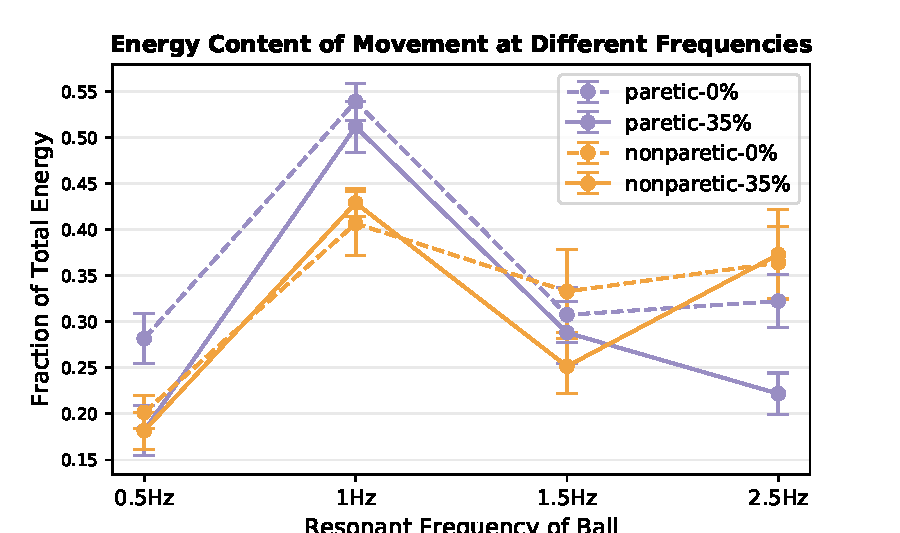
\includegraphics[width=0.5\linewidth]{Plots/IndividualSubjectPlots/S208/S208.pdf}}
	\caption{Subject 208 Frequency Spectrums. Interation effect between arm and ball frequency (p$<$0.001). Loading is a significant factor (p$<$0.05). For the 1Hz and 2.5Hz ball, arm is a significant factor, p$<$0.001 and p$<$0.05 respectively. For the 0.5Hz and 2.5Hz ball, loading is a significant factor in the paretic arm (p$<$0.05).}
\end{figure}

\clearpage
\subsection{S209; FMA = 49}

\begin{figure}[!ht]
     \centering
     \subfloat{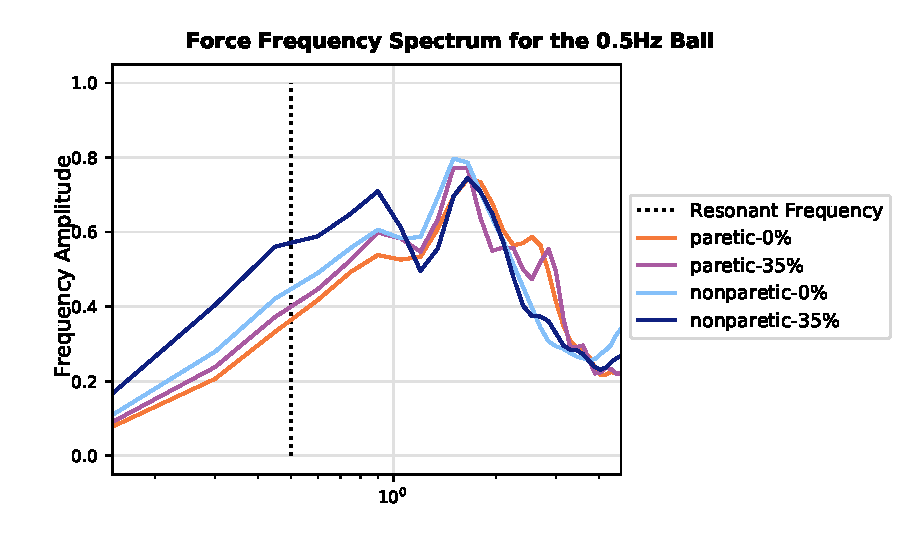
\includegraphics[width=0.5\linewidth]{Plots/IndividualSubjectPlots/S209/S209_0.5Hz.pdf}}
     \subfloat{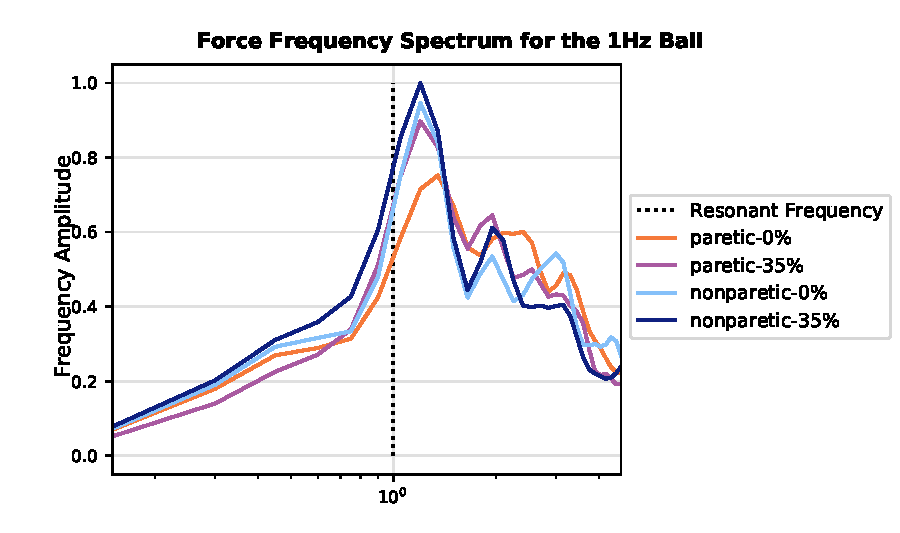
\includegraphics[width=0.5\linewidth]{Plots/IndividualSubjectPlots/S209/S209_1Hz.pdf}}
     \hfill
     \subfloat{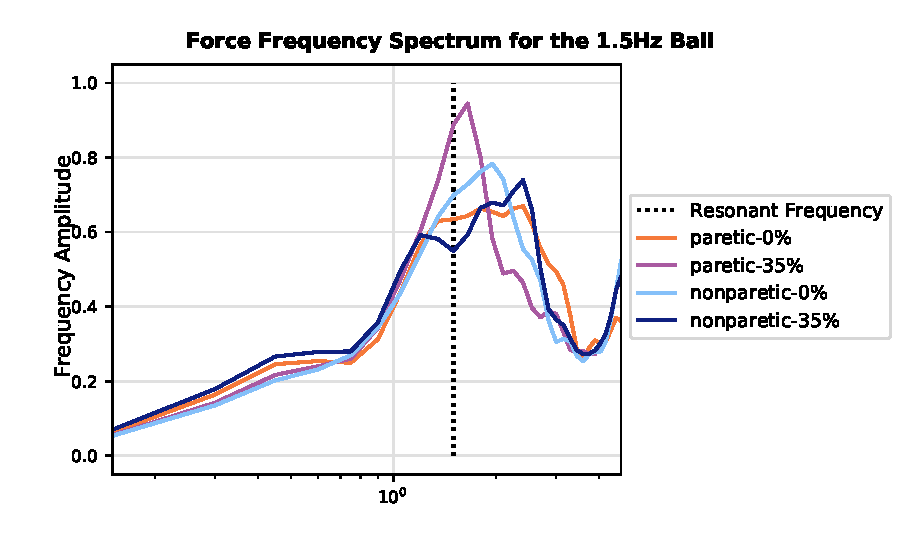
\includegraphics[width=0.5\linewidth]{Plots/IndividualSubjectPlots/S209/S209_1.5Hz.pdf}}
     \subfloat{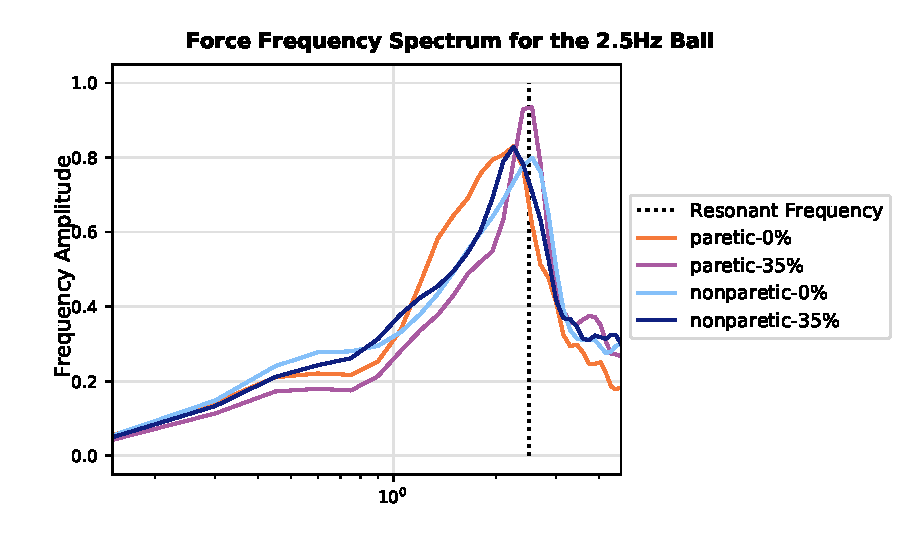
\includegraphics[width=0.5\linewidth]{Plots/IndividualSubjectPlots/S209/S209_2.5Hz.pdf}}
     \hfill
     \subfloat{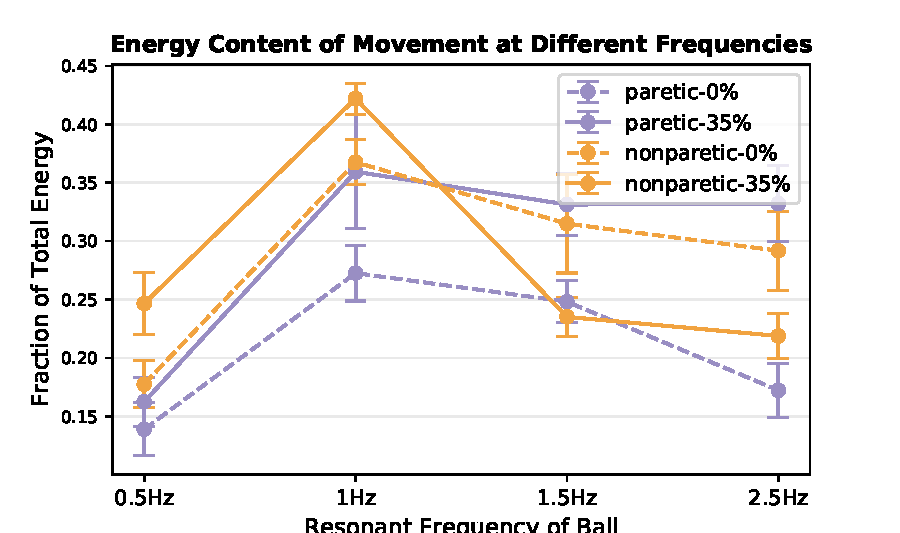
\includegraphics[width=0.5\linewidth]{Plots/IndividualSubjectPlots/S209/S209.pdf}}
	\caption{Subject 209 Frequency Spectrums. Interation effect between arm and ball frequency (p$<$0.05). Arm and loading are significant factors. Interaction effect between arm, ball frequency, and loading....pretty much everything is significant.}
\end{figure}


\clearpage
\subsection{S211; FMA = 17}

\begin{figure}[!ht]
     \centering
     \subfloat{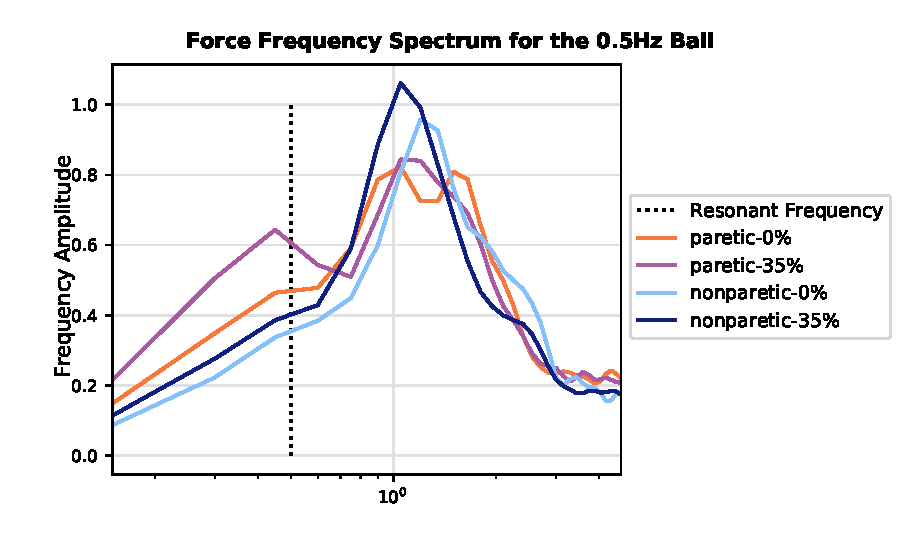
\includegraphics[width=0.5\linewidth]{Plots/IndividualSubjectPlots/S211/S211_0.5Hz.pdf}}
     \subfloat{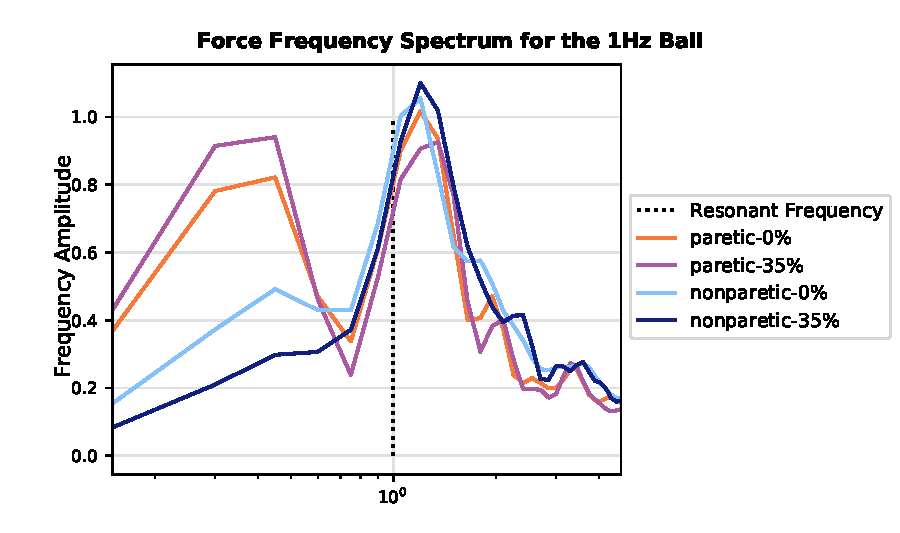
\includegraphics[width=0.5\linewidth]{Plots/IndividualSubjectPlots/S211/S211_1Hz.pdf}}
     \hfill
     \subfloat{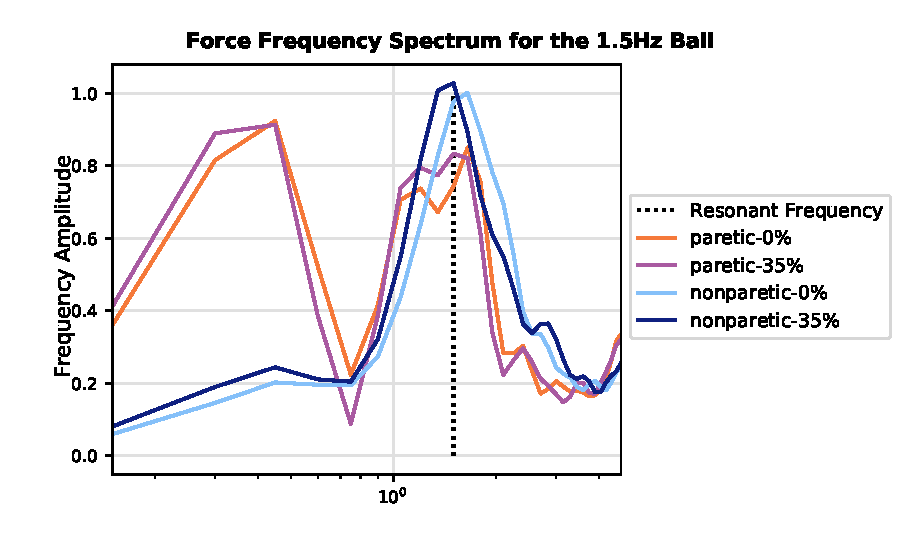
\includegraphics[width=0.5\linewidth]{Plots/IndividualSubjectPlots/S211/S211_1.5Hz.pdf}}
     \subfloat{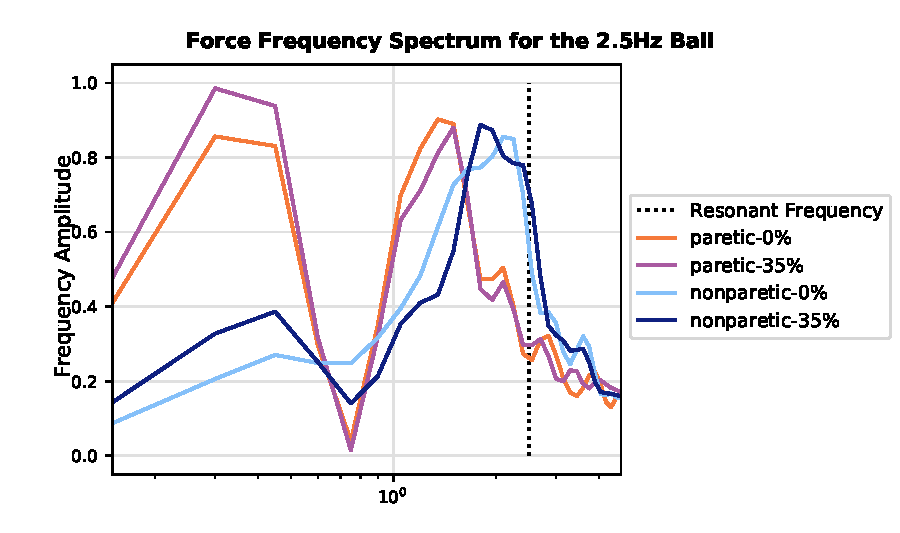
\includegraphics[width=0.5\linewidth]{Plots/IndividualSubjectPlots/S211/S211_2.5Hz.pdf}}
     \hfill
     \subfloat{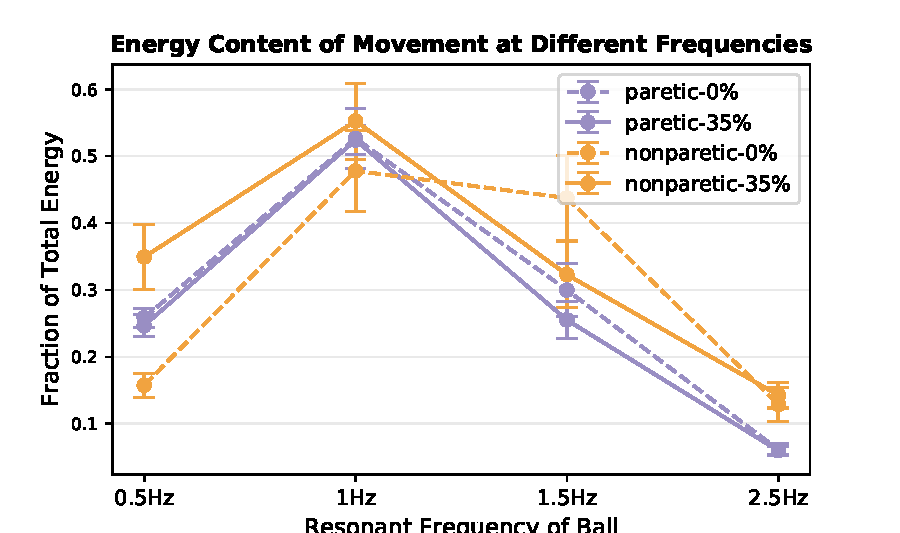
\includegraphics[width=0.5\linewidth]{Plots/IndividualSubjectPlots/S211/S211.pdf}}
	\caption{Subject 211 Frequency Spectrums. Interation effect between loading and ball frequency (p$<$0.05). For the 2.5Hz ball, arm is a significant factor. }
\end{figure}

\clearpage
\subsection{S212; FMA = 13}

\begin{figure}[!ht]
     \centering
     \subfloat{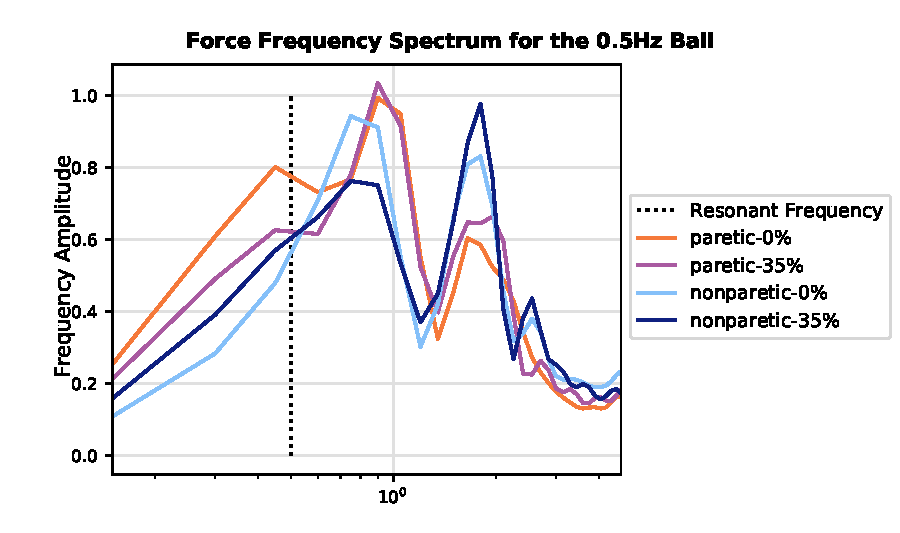
\includegraphics[width=0.5\linewidth]{Plots/IndividualSubjectPlots/S212/S212_0.5Hz.pdf}}
     \subfloat{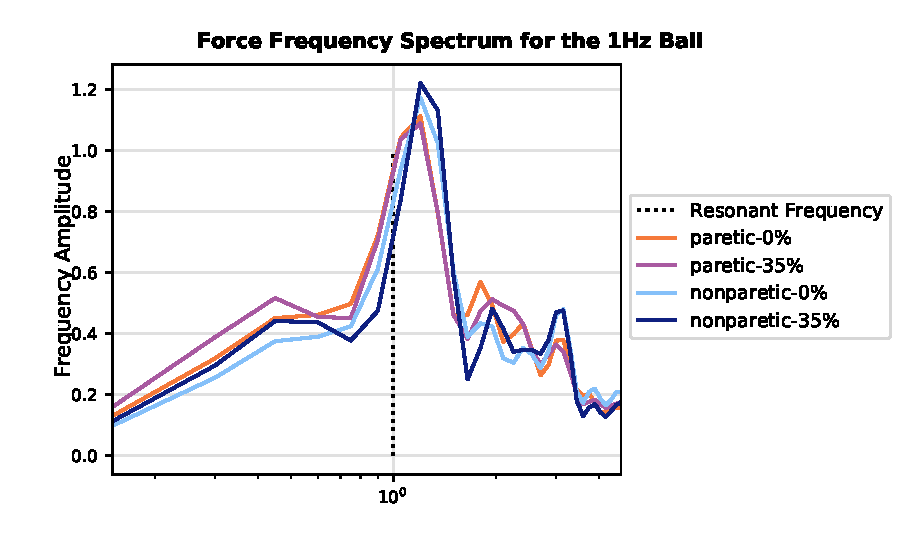
\includegraphics[width=0.5\linewidth]{Plots/IndividualSubjectPlots/S212/S212_1Hz.pdf}}
     \hfill
     \subfloat{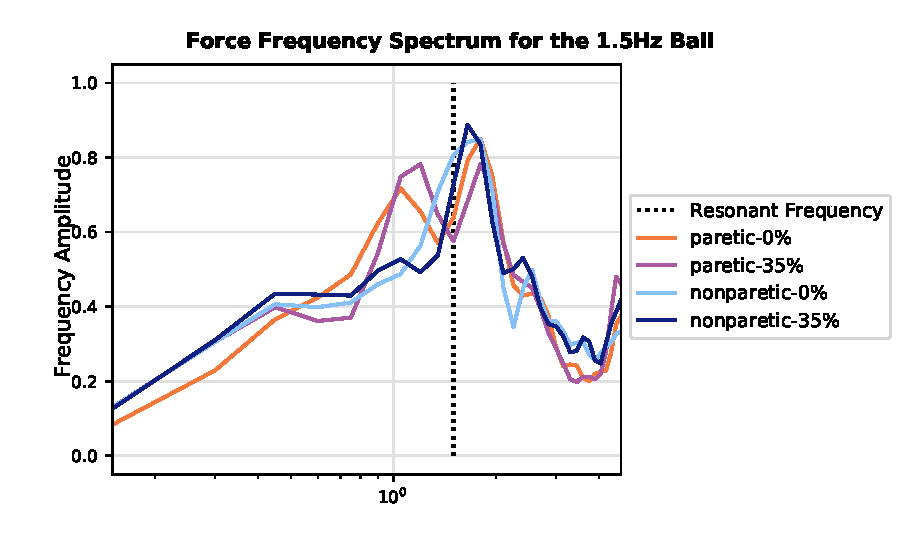
\includegraphics[width=0.5\linewidth]{Plots/IndividualSubjectPlots/S212/S212_1.5Hz.pdf}}
     \subfloat{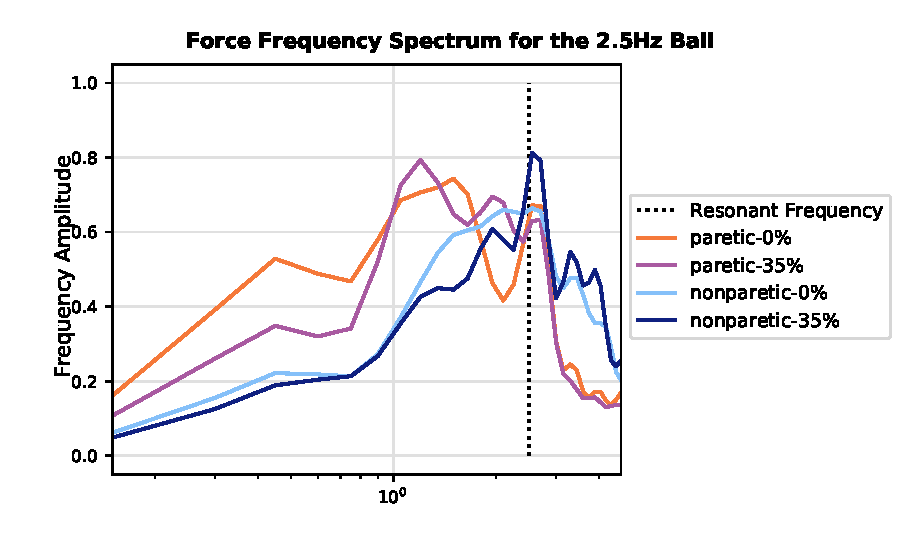
\includegraphics[width=0.5\linewidth]{Plots/IndividualSubjectPlots/S212/S212_2.5Hz.pdf}}
     \hfill
     \subfloat{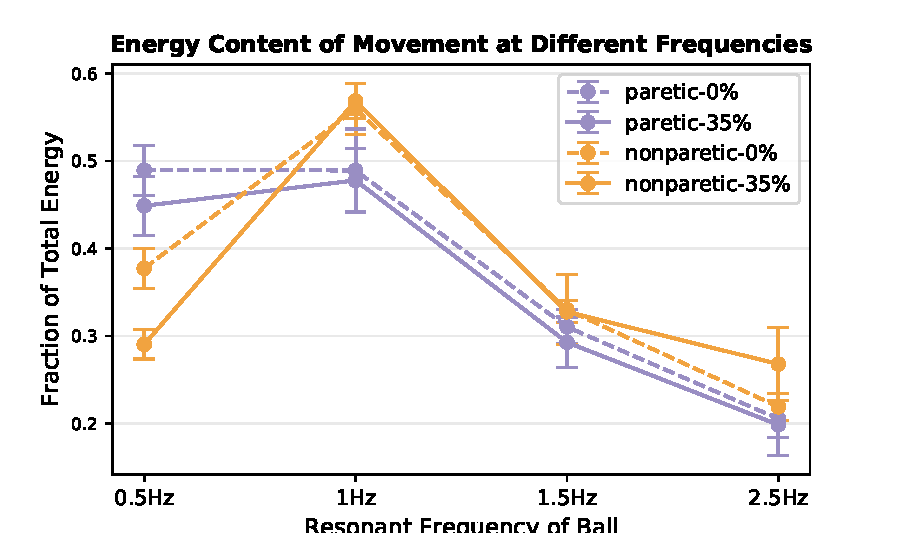
\includegraphics[width=0.5\linewidth]{Plots/IndividualSubjectPlots/S212/S212.pdf}}
	\caption{Subject 212 Frequency Spectrums. Interation effect between arm and ball frequency (p$<$0.001). For the 0.5Hz and 1Hz balls, arm is a significant factor. Ball frequency is a significant factor for percent decrease in paretic arm with loading  with 0.5Hz being different.}
\end{figure}

\end{document}